% Canonical caption for figCalculusPanels.pdf
% Generated by: code/paper0/course_panels_figure.py from
% mart.course_poverty (GATEWAY) and figAlgebraIIOA_data.csv.
\begin{figure}[tbp]
  \centering
  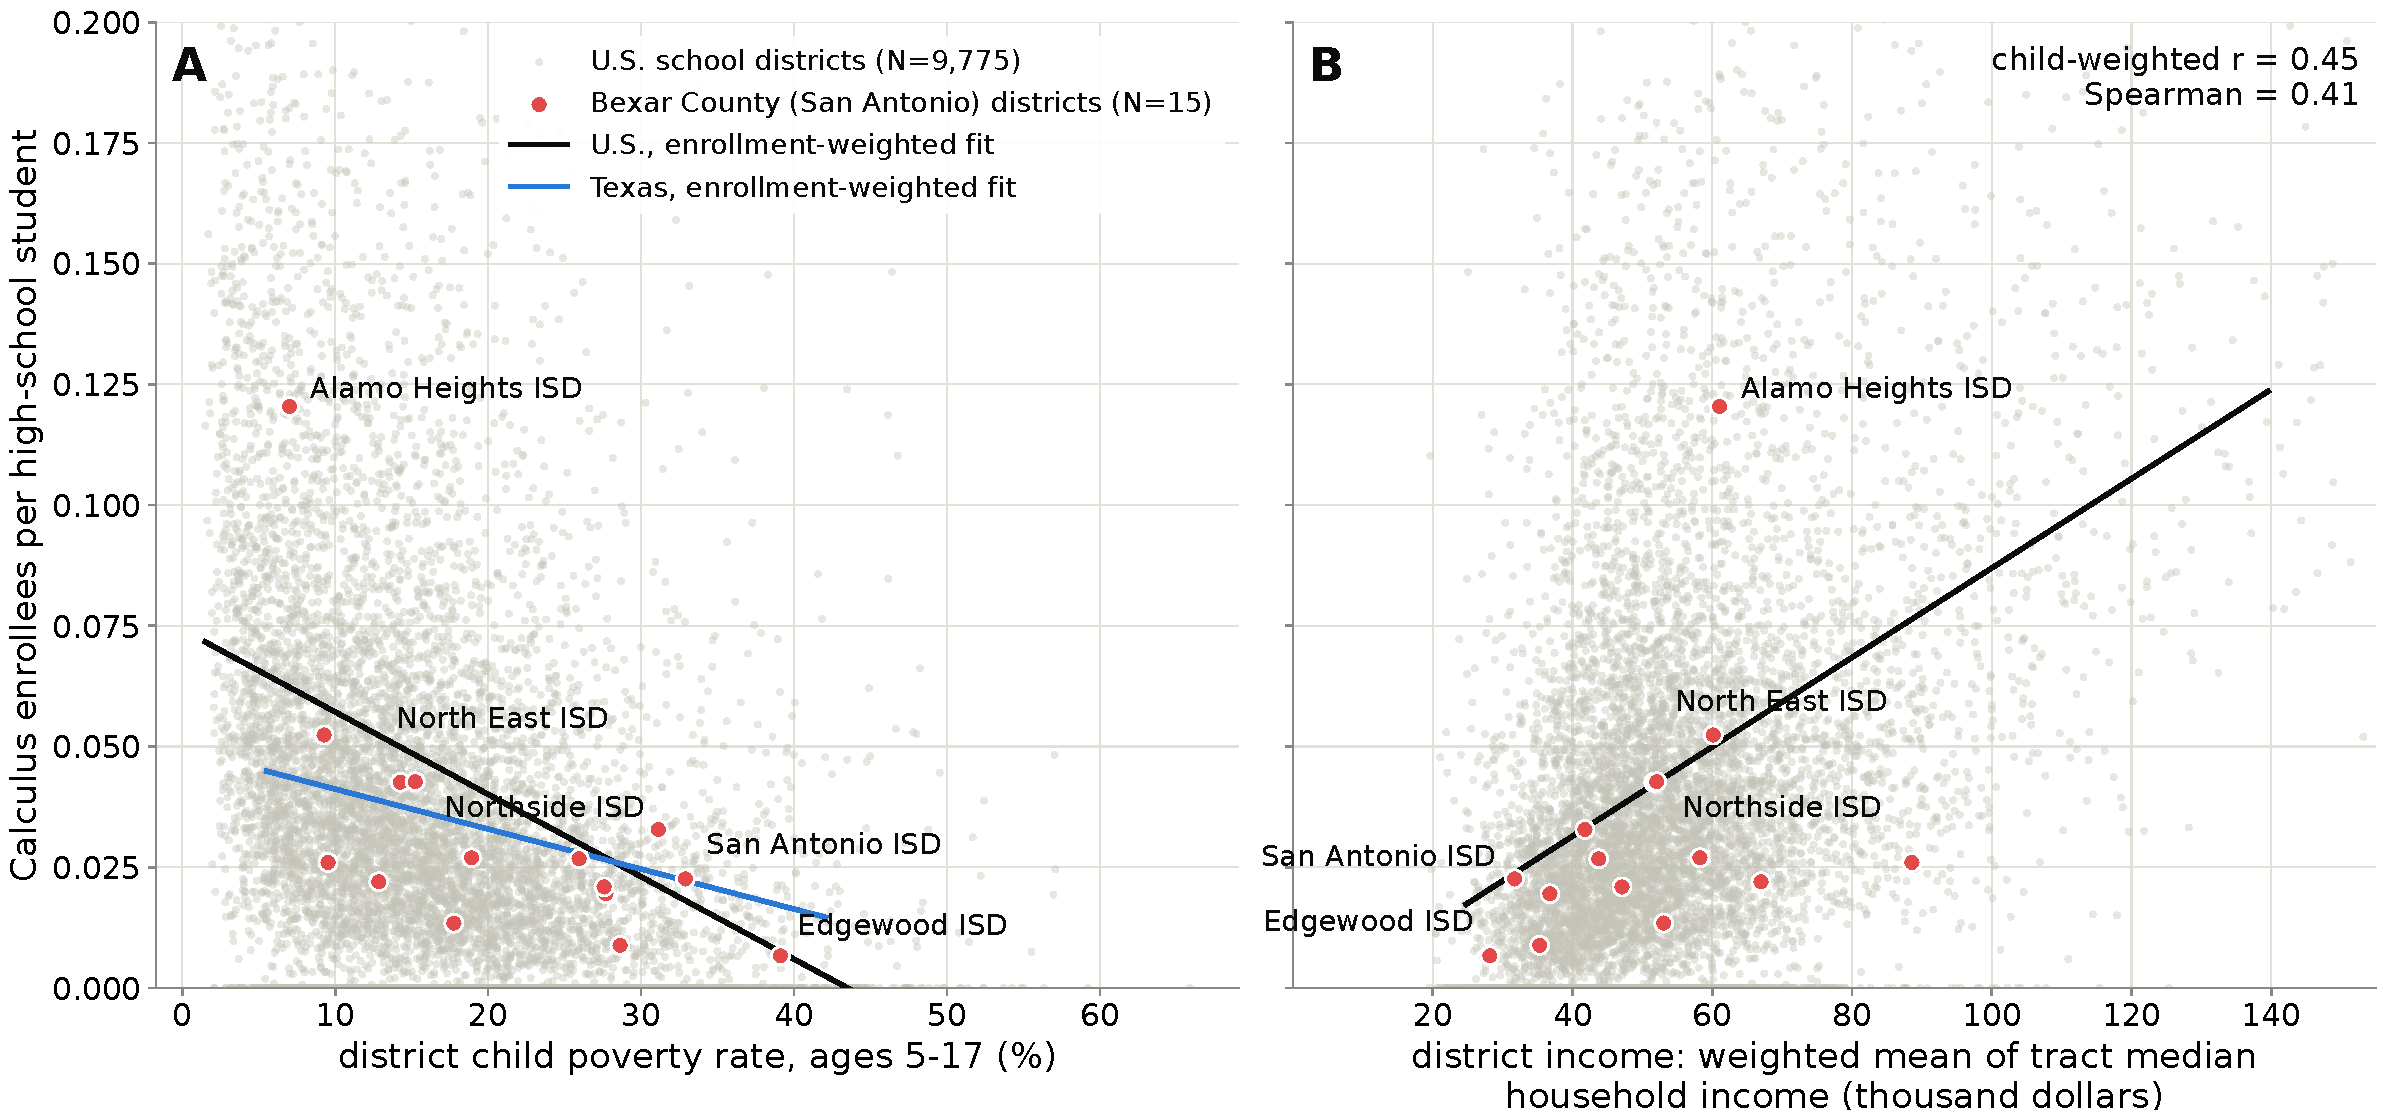
\includegraphics[width=\textwidth]{figCalculusPanels.pdf}
  \caption{District Calculus enrollment per high-school
    student (CRDC 2017--18) against (A) the district child poverty
    rate (SAIPE 2017) and (B) district income, the weighted mean of
    tract median household incomes (ACS 2012--16, the tract
    covariate distributed with the Opportunity Atlas; tracts
    weighted by childhood-cohort count times land-area share), for
    the 9,790 districts of the
    common frame (matched, at least 200 children aged 5--17,
    a high-school course sequence reported, no missing-coded
    course item). The denominator is estimated high-school
    enrollment: total enrollment of the schools serving grades
    9--12, prorated by grade span. (A) The black line is the U.S.
    enrollment-weighted least-squares fit, slope $-0.171$ per
    unit of the poverty rate (state-clustered standard error
    0.020), which is $-36.9\%$ of the national mean
    (0.046) per ten percentage points of child poverty; the
    blue line is
    the same fit within Texas (860 districts). (B) The
    9,775 districts with an income value; the
    child-weighted correlation is 0.45 (Spearman 0.41).
    Red: the school districts of Bexar County, Texas (15 in the
    frame, landmark districts labeled).
    2,321 districts report no Calculus enrollment, and 112
    above the displayed range are not shown. Districts are the
    units; enrollment counts seats within one cycle, with no
    completion or outcome content.}
  \label{figCalculusPanels}
\end{figure}
